\chapter{Results}\label{results}
\section{Timing}
% May want criterion timing info
The timing tests have been split into three tests: one for the greedy solvers; one for the simulated annealing, adaptive annealing and late acceptance hill climbing; and one for the parallel tempering solver. The timing test for the greedy solvers can be seen in Figure~\ref{greedy_time}. This figure shows the amount of ICCs which have been calculated for constructive algorithms of various beam sizes against their runtime in seconds. There is a strong linear correlation between these two variables. A linear fit through these points gives a slope of \(1.71\cdot 10^{-3} \pm 7.06\cdot 10^{-6}\ s\ \text{ICC}^{-1}\), which is about 585 ICCs per second, and an intercept of \(0.34 \pm 0.024\ \text{ICCs}\). 

The timing test for the serial Metropolis solvers can be seen in Figure~\ref{annealing_time}. Here the correlation between runtime and ICCs calculated appears to contain more noise, but a clear linear relation can still be seen. A linear fit through these points gives a slope of \(3.09\cdot 10^{-3} \pm 5.9\cdot 10^{-5}\ s\ \text{ICC}^{-1}\), which is about 323 ICCs per second, and an intercept of \(-2.6 \pm 1.24\ \text{ICCs}\). The Metropolis step based solvers appear to run slower per ICC calculated than the greedy solvers, possibly due to some inefficiency in computing resource usage. The cause of this slowdown or the source of the additional noise in the solver runtime has not been investigated in this thesis.

The timing test for the parallel tempering solvers can be seen in Figure~\ref{parallel_time}. Here the linear correlation may appear less clear, but a linear fit still reveals a linear relation between the runtime and ICCs calculates. The fit gives a slope of \(3.7\cdot 10^{-4} \pm 3.49\cdot 10^{-5}\ s\ \text{ICC}^{-1}\), which is about 2703 ICCs per second, and an intercept of \(-53.4 \pm 17.9\ \text{ICCs}\). This solver has a higher throughput of ICCs per second than the other two solvers, but this number does not yet take into account that this solver runs on all of the threads of the computers CPU.\@ 

\begin{figure}
  \centering
  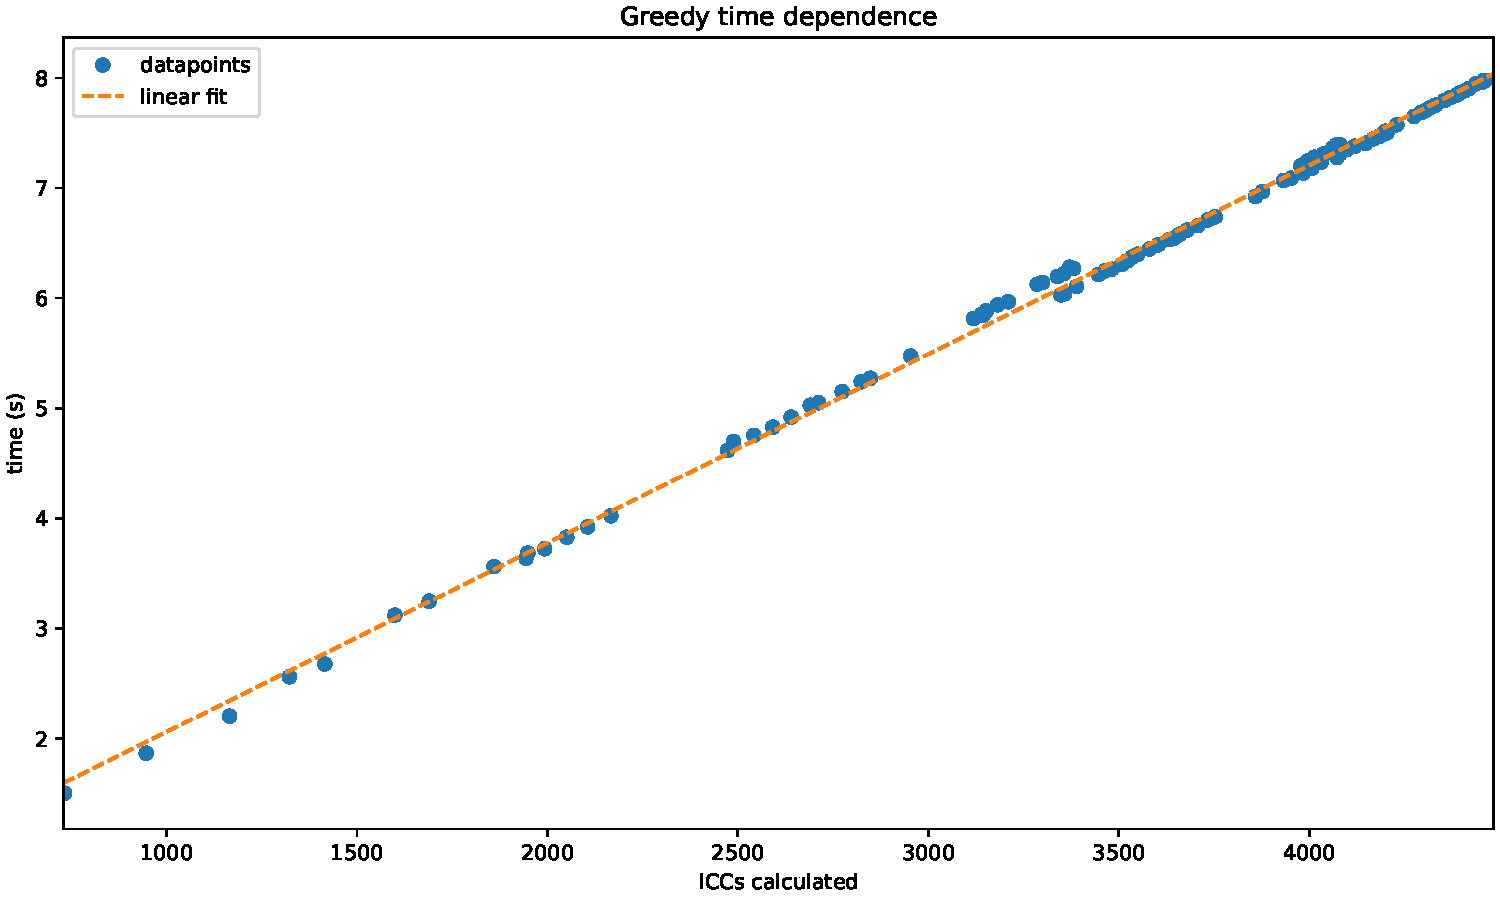
\includegraphics[width=\textwidth]{./Figures/Greedy_time_dependence.pdf}
  \caption{The amount of ICCs which have been calculated for constructive algorithms of various beam sizes against their runtime in seconds. There is a strong linear correlation between these two variables. A linear fit through these points gives a slope of \(1.71\cdot 10^{-3} \pm 7.06\cdot 10^{-6}\ s\ \text{ICC}^{-1}\), which is about 585 ICCs per second, and an intercept of \(0.34 \pm 0.024\ \text{ICCs}\). }\label{greedy_time}
\end{figure}
\begin{figure}
  \centering
  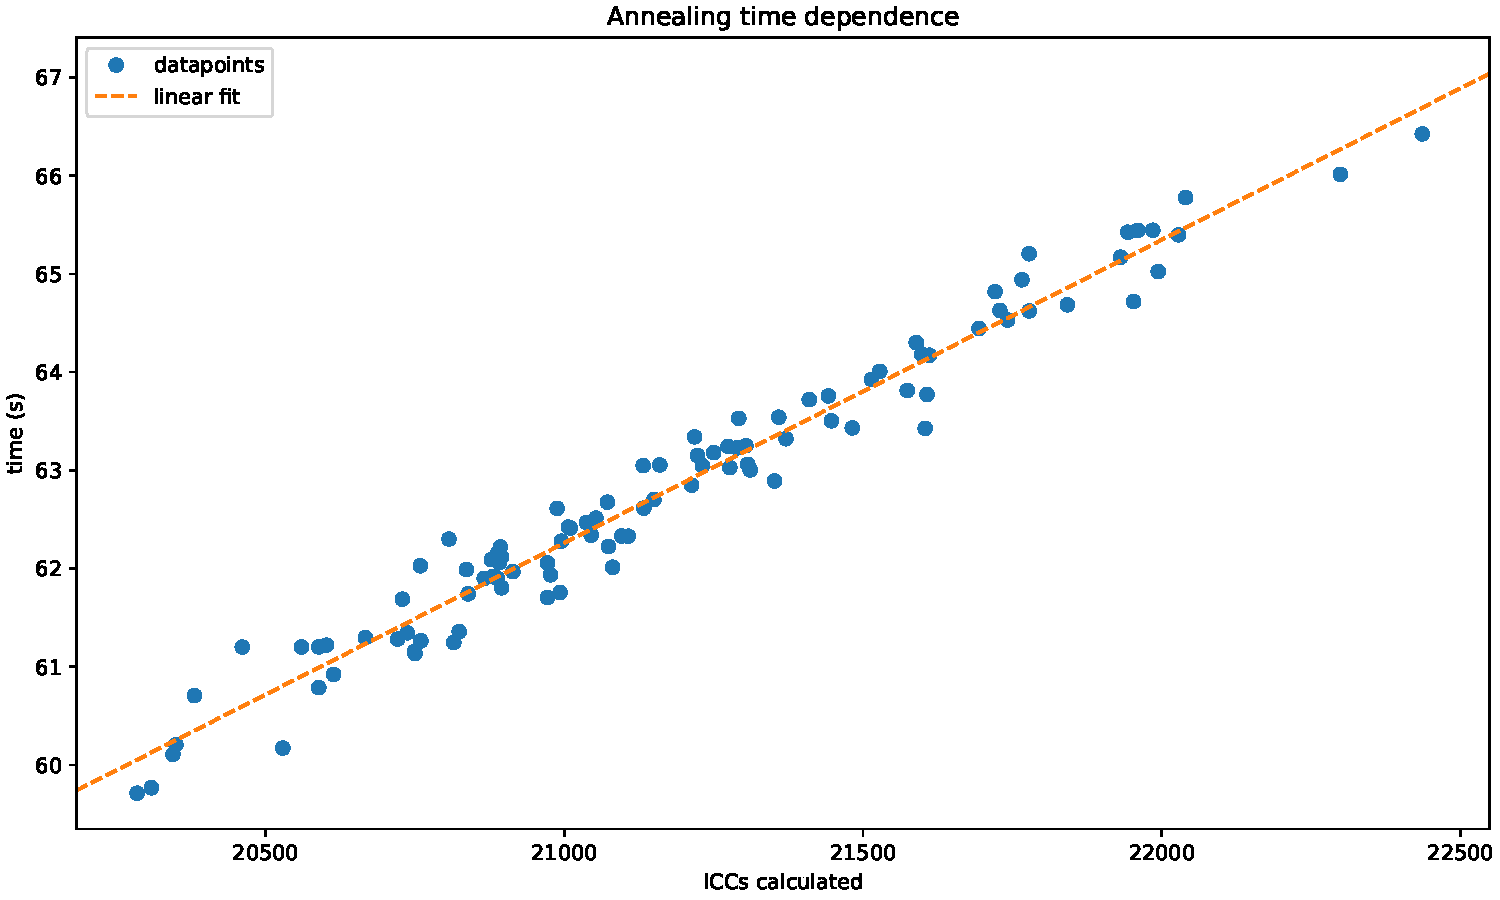
\includegraphics[width=\textwidth]{./Figures/Annealing_time_dependence.pdf}
  \caption{The amount of ICCs which have been calculated by different runs of a simulated annealing algorithm against their runtime in seconds. Here the correlation between runtime and ICCs calculated appears to contain more noise, but a clear linear relation can still be seen. A linear fit through these points gives a slope of \(3.09\cdot 10^{-3} \pm 5.9\cdot 10^{-5}\ s\ \text{ICC}^{-1}\), which is about 323 ICCs per second, and an intercept of \(-2.6 \pm 1.24\ \text{ICCs}\).}\label{annealing_time}
\end{figure}
\begin{figure}
  \centering
  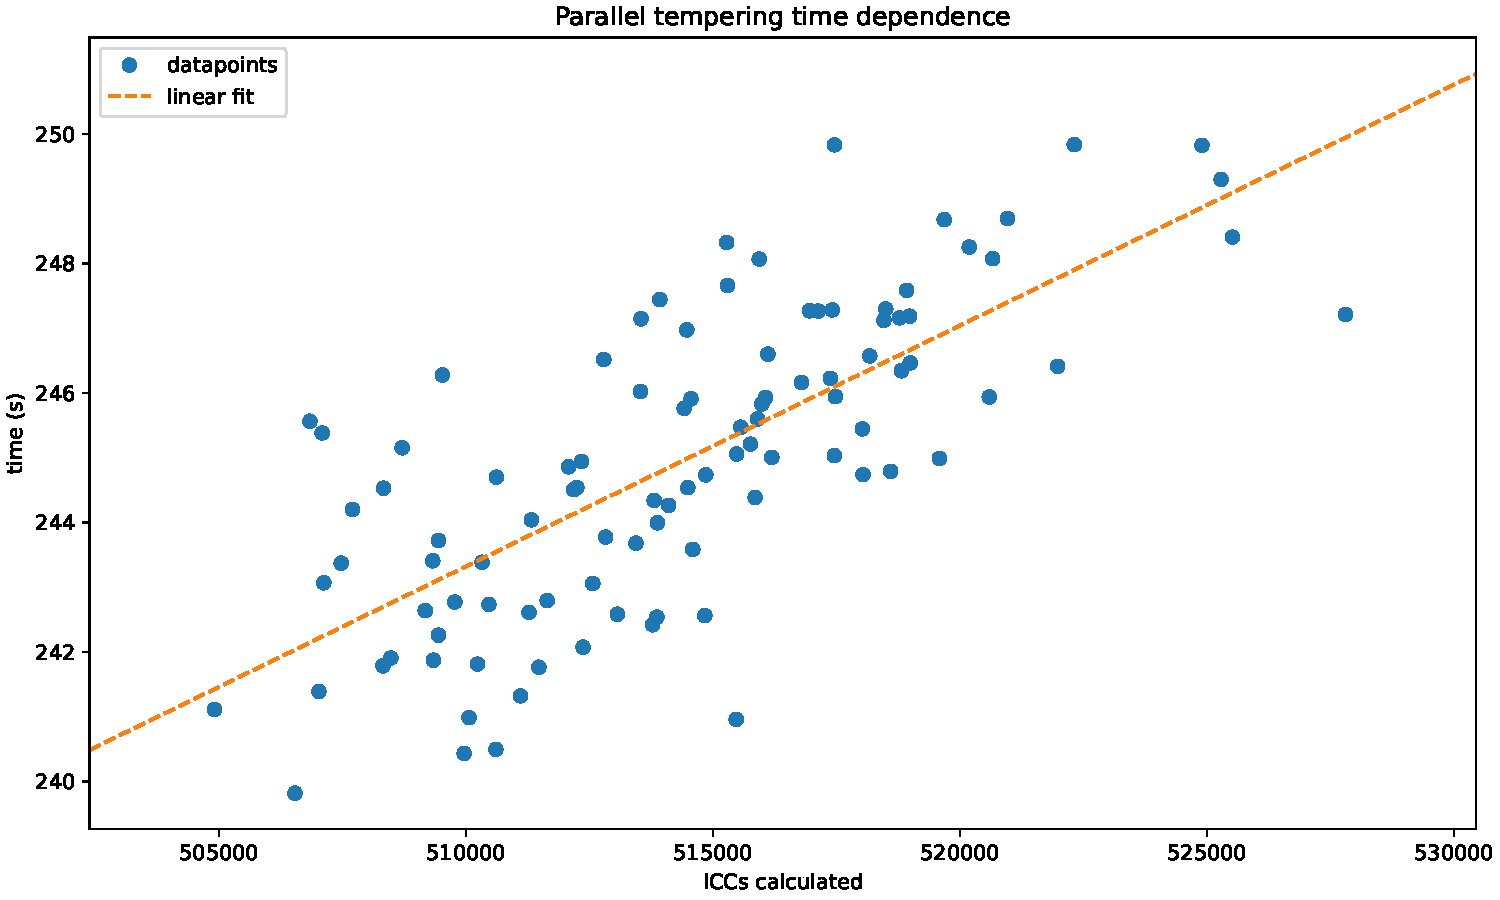
\includegraphics[width=\textwidth]{./Figures/Parallel tempering_time_dependence.pdf}
  \caption{The amount of ICCs which have been calculated by different runs of a parallel tempering algorithm against their runtime in seconds. Here the linear correlation may appear less clear, but a linear fit still reveals a linear relation between the runtime and ICCs calculates. The fit gives a slope of \(3.7\cdot 10^{-4} \pm 3.49\cdot 10^{-5}\ s\ \text{ICC}^{-1}\), which is about 2703 ICCs per second, and an intercept of \(-53.4 \pm 17.9\ \text{ICCs}\).}\label{parallel_time}
\end{figure}

A summary of these results can be found in Table~\ref{timing_summary}. Of the three solvers measured here, the parallel tempering manages to process the most ICCs per second, as this algorithm processes 4.62 times more ICCs per second than the greedy algorithm and 8.37 times more than the annealing algorithm. This does not take into account that this algorithm is inherently multithreaded, however. This test was run on an AMD r5 7600, which has 6 cores and 12 threads. The parallel tempering algorithm therefore should have a six to twelve times higher throughput than an equivalent serial algorithm. When the throughput of this algorithm is compensated for the amount of cores, the algorithm 

\begin{table}[b!]
    \centering
    \caption{A summary of the timing tests. The parallel tempering algorithm is included both unedited and with compensation for the six CPU cores it was measured on.}
    \begin{tabular}{rccc}
    \toprule
        Solver & seconds per ICC & ICC per second & Relative speed \\
    \midrule
        Greedy & \(1.71\cdot 10^{-3} \pm 7.06\cdot 10^{-6}\) & 585 & 1.0x\\
        Simulated annealing & \(3.09\cdot 10^{-3} \pm 5.9\cdot 10^{-5}\) & 323 & 0.55x\\
        Parallel tempering & \(3.7\cdot 10^{-4} \pm 3.49\cdot 10^{-5}\) & 2703 & 4.62x\\
        % I cheated on the error here.
        PT core compensated & \(2.22\cdot 10^{-3} \pm 2.09\cdot 10^{-4}\) & 450 & 0.77x\\
    \bottomrule
    \end{tabular}
    \label{timing_summary}
\end{table}